\documentclass[conference]{IEEEtran}
\usepackage[T1]{fontenc}
\usepackage{cite}
\usepackage{graphicx}
\usepackage{booktabs}
\usepackage{xcolor}
\usepackage{microtype}
\usepackage{tikz}
\usetikzlibrary{arrows.meta,positioning,fit,calc}
\usepackage{pgfplots}
\pgfplotsset{compat=1.18}
\usepackage[hidelinks]{hyperref}

\definecolor{okgreen}{RGB}{46,139,87}
\definecolor{failred}{RGB}{196,64,64}
\definecolor{unkgray}{RGB}{200,200,200}
\definecolor{boxblue}{RGB}{225,236,250}
\definecolor{edgeblue}{RGB}{40,90,160}

\begin{document}
\raggedbottom

\title{Robot Learning for Household Tasks: SO101 Demonstrations, OriginX Adaptation, and Training-Free Execution}

\author{\IEEEauthorblockN{Qinzhen Ma}
\IEEEauthorblockA{MECE Program, Department of Electrical and Computer Engineering, Rice University\\
ELEC 594 Capstone, Fall 2026 --- Midterm Report\\
qm18@rice.edu}}

\maketitle

\begin{abstract}
Household manipulation requires a robot to know which object to manipulate, which task stage it is in, and whether that stage is complete. We study these problems in two tracks. On a real SO101 arm, we recorded demonstrations of three household tasks and built a 102-episode cube-into-cup dataset in LeRobot format. In RoboCasa365 simulation, we adapted the Xiaomi-Robotics-1 vision-language-action policy with an Action LoRA and a 4.22M-parameter conditioning branch; an author-run evaluation reached 1,496/2,500 successes (59.84\%), but a matched comparison showed no clear gain. We then built OriginX-TF, a training-free harness that adds object identity, stage contracts and visual verification around a frozen policy. It runs unchanged with two frozen policies and passes 145 CPU tests. A pilot (12 of 14 episodes completed) shows no success gain yet and points to identity recovery and stage verification as bottlenecks.
\end{abstract}

\section{Introduction}
Robots that help in homes must handle rigid, deformable and articulated objects, and they must keep track of task progress over long horizons. Recent vision-language-action (VLA) policies map camera images, a language instruction and the robot state directly to actions~\cite{xiaomi2026robotics1}. When such a policy fails, the failure is not always a low-level motion error: the policy may act on the wrong object, repeat a finished stage, or move on before a stage is done. Language-model planners~\cite{ahn2022saycan,huang2022inner} and recent harnesses around frozen VLA policies~\cite{li2026roboharness,gao2026agm} decompose a task and check its progress outside the policy.

This project follows two tracks (Fig.~\ref{fig:so101} illustrates the first and Fig.~\ref{fig:harness} part of the second). The \emph{real-robot track} builds a data and training pipeline on a low-cost SO101 arm~\cite{so101arm} with LeRobot~\cite{cadene2024lerobot}. The \emph{simulation track} uses the RoboCasa365 kitchen benchmark~\cite{nasiriany2024robocasa,nasiriany2026robocasa365}, where initial states can be controlled and closed-loop success is measured by the environment. At the midterm, the project has produced: (i) teleoperated demonstrations of three household tasks and a LeRobot dataset for one of them; (ii) an adapted Xiaomi-Robotics-1 policy (OriginX) with a complete 2,500-episode evaluation~\cite{ma2026originx}; and (iii) OriginX-TF, a training-free execution harness that runs with two different frozen policies. The engineering results are verified; a task-success improvement is not yet shown, and we state this limit explicitly.

\section{Methods}

\subsection{SO101 Demonstration Pipeline}
The SO101 follower arm has five revolute joints and a gripper (six position-controlled actuators: shoulder pan, shoulder lift, elbow flex, wrist flex, wrist roll and gripper). Demonstrations are recorded by teleoperation with a leader arm. We recorded three tasks that cover different object types: placing a cube into a cup (rigid object), folding clothes (deformable object) and closing a toolbox (articulated object). The cube task is organized as a LeRobot v3 dataset in which each frame stores the six-dimensional joint state, the six-dimensional action, and one $640\times480$ RGB image from each of two cameras (front and wrist), at 30\,Hz (Fig.~\ref{fig:so101}). As a first policy baseline, we trained an Action Chunking Transformer (ACT)~\cite{zhao2023act} with a chunk size of 100 for 30k steps on the 100 cube episodes available at the time.

\begin{figure*}[t]
  \centering
  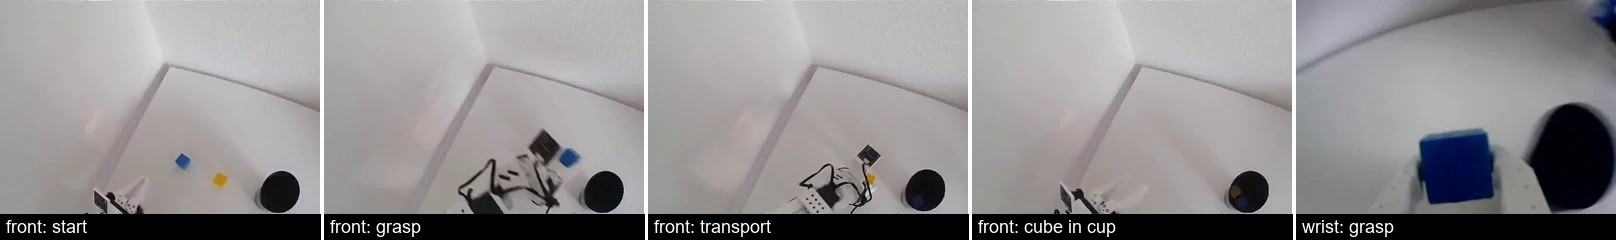
\includegraphics[width=\textwidth]{figures/so101_frames.jpg}
  \caption{One recorded SO101 demonstration (episode 0 of the 102-episode cube-into-cup dataset, 912 frames). Four front-camera frames from start to placement and one wrist-camera frame at the grasp. Clothes folding and toolbox closing were also recorded on SO101; they are not included in these dataset statistics.}
  \label{fig:so101}
\end{figure*}

\subsection{OriginX: Adapting a Frozen VLA Policy}
Xiaomi-Robotics-1~\cite{xiaomi2026robotics1} combines a vision-language backbone with a flow-based action transformer. We start from its public RoboCasa365 checkpoint. In Stage~A we adapt the action model with a low-rank adapter (Action LoRA)~\cite{hu2022lora}. In Stage~B we freeze the adapted policy and train a 4.22M-parameter conditioning branch that uses vision-language features and recent robot state to condition action generation. A stage-prediction objective is used during training only; it is not an input at test time.

\subsection{OriginX-TF: A Training-Free Execution Harness}
OriginX-TF moves stage management outside the policy and makes no parameter updates (Fig.~\ref{fig:harness}). It has four parts.

\emph{Object identity.} A frozen OWLv2 detector~\cite{minderer2023owlv2} proposes kitchen-object candidates, and a causal tracker uses frozen CLIP~\cite{radford2021clip} appearance features to associate them over time, keeping up to 32 candidates with persistent track IDs. These IDs are visual handles, not simulator ground truth.

\emph{Stage contracts.} Before the first action, a frozen Qwen3-VL-4B-Instruct model~\cite{qwen3vl4b} reads the task, the three camera views and the candidates, and writes one to four contracts. Each contract has a stage instruction (e.g., ``pick up the mug''), a target ID, and a visual postcondition for that stage only.

\emph{Visual verification.} Every 64 control steps, the same frozen model compares the three stage-reference views with the three current views and checks the bound target and the postcondition. The state machine advances only after two consistent confirmations at different times.

\emph{Portable policy interface.} The harness reads the public observations (three RGB views, proprioception and the instruction), passes the current stage instruction as natural language, and resets the policy's history when the instruction changes. The policy's native action chunk (16 steps $\times$ 12 action dimensions) is executed without modification. If the bound target is not visible, the harness falls back to the original task instruction. Task success is always decided by the environment's evaluator, not by the harness. The same harness is connected to Xiaomi-Robotics-1 and to Awomo-0.5I~\cite{awomo2026}, each with its own frozen checkpoint.

\begin{figure}[t]
\centering
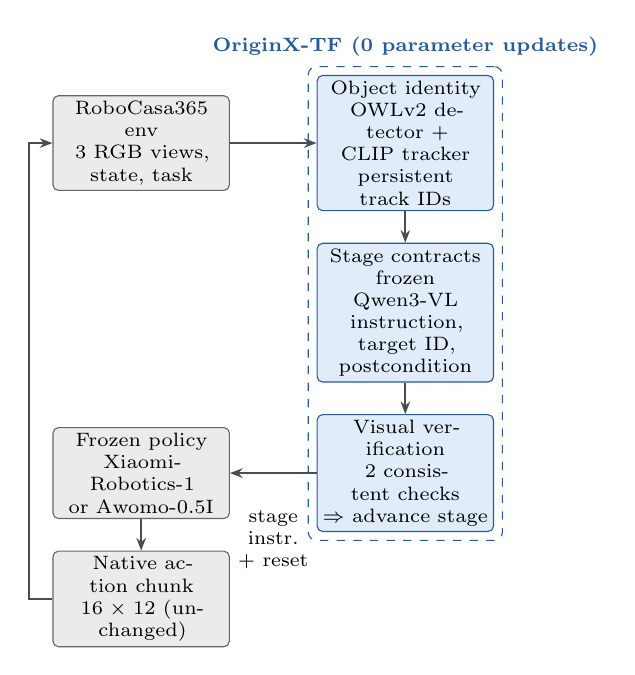
\begin{tikzpicture}[
  font=\scriptsize,
  box/.style={draw=edgeblue, fill=boxblue, rounded corners=2pt, align=center, minimum height=7mm, inner sep=2pt},
  fz/.style={draw=black!60, fill=black!8, rounded corners=2pt, align=center, minimum height=7mm, inner sep=2pt},
  arr/.style={-{Stealth[length=1.6mm]}, thick, black!70}]
  \node[fz, text width=21mm] (env) {RoboCasa365 env\\3 RGB views, state, task};
  \node[box, text width=21mm, right=11mm of env] (track) {Object identity\\OWLv2 detector +\\CLIP tracker\\persistent track IDs};
  \node[box, text width=21mm, below=4mm of track] (plan) {Stage contracts\\frozen Qwen3-VL\\instruction, target ID,\\postcondition};
  \node[box, text width=21mm, below=4mm of plan] (ver) {Visual verification\\2 consistent checks\\$\Rightarrow$ advance stage};
  \node[fz, text width=21mm, left=11mm of ver] (pol) {Frozen policy\\Xiaomi-Robotics-1\\or Awomo-0.5I};
  \node[fz, text width=21mm, below=4mm of pol] (act) {Native action chunk\\$16\times12$ (unchanged)};
  \draw[arr] (env) -- (track);
  \draw[arr] (track) -- (plan);
  \draw[arr] (plan) -- (ver);
  \draw[arr] (ver) -- (pol);
  \node[below=0.5mm of $(ver.west)!0.5!(pol.east)$, align=center, font=\scriptsize, yshift=-3mm] {stage\\instr.\\+ reset};
  \draw[arr] (pol) -- (act);
  \draw[arr] (act.west) -- ++(-3mm,0) |- (env.west);
  \node[draw=edgeblue, dashed, rounded corners=3pt, inner sep=3pt, fit=(track)(plan)(ver), label={[font=\scriptsize\bfseries, text=edgeblue]above:OriginX-TF (0 parameter updates)}] {};
\end{tikzpicture}
\caption{OriginX-TF wraps a frozen policy. Blue blocks are the harness; gray blocks are unchanged components. All models are frozen.}
\label{fig:harness}
\end{figure}

\subsection{Evaluation Protocol}
For the earlier adaptation study we ran 50 RoboCasa365 tasks with 50 episodes each. For OriginX-TF we ran a small fixed pilot on two tasks, CoffeeSetupMug (coffee) and PickPlaceCounterToCabinet (cabinet), with one seed per task and seven experimental arms: native Xiaomi, Xiaomi with the full harness, three Xiaomi ablations (\emph{no-stage}: no stage instructions or their history resets; \emph{no-binding}: no identity/visibility gating; \emph{single-confirm}: one confirmation instead of two), native Awomo, and Awomo with the full harness. This gives 14 planned episodes. Comparisons are made only between episodes with matching initial-state fingerprints, and episodes without a terminal result stay in the denominator as \emph{unknown}. All harness runs used a single RTX 5090 Laptop GPU with 24\,GB of memory, loading the models sequentially.

\section{Results (Partial)}

\subsection{Real-Robot Data}
The cube-into-cup dataset contains 102 episodes and 65,620 frames (mean 643 frames, about 21\,s per episode) with front and wrist video (Fig.~\ref{fig:so101}). ACT training finished all 30k steps; its closed-loop success on the real arm is not yet reported.

\subsection{OriginX Adaptation in RoboCasa365}
The full author-run evaluation of the stage-supervised model finished all 2,500 episodes with 1,496 successes (59.84\%). This is our own evaluation, not an official leaderboard entry. To test whether the added branch helps, we ran a separate 50-case comparison (Fig.~\ref{fig:robocasa}). Raw successes were 30/50 for the base policy, 32/50 for Action LoRA and 33/50 for OriginX. Among 44 matched LoRA/OriginX pairs, OriginX won 5, lost 4 and tied 35; 6 comparisons are unresolved. The added benefit of the branch is therefore uncertain.

Two failure studies motivated the harness. Supplying one language subgoal from gpt-6-astra (high reasoning effort, given the three current views) to the frozen OriginX policy produced 56 verified rescues (failures turned into successes) among 1,004 historical failures~\cite{ma2026originx}. In a visual-grounding pilot with the frozen base Xiaomi policy, an oracle-placed (correct) visual cue versus the raw input gave 3 wins and 1 loss over 45 matched cases, with 3 of 48 planned cases unresolved.

\begin{figure}[t]
\centering
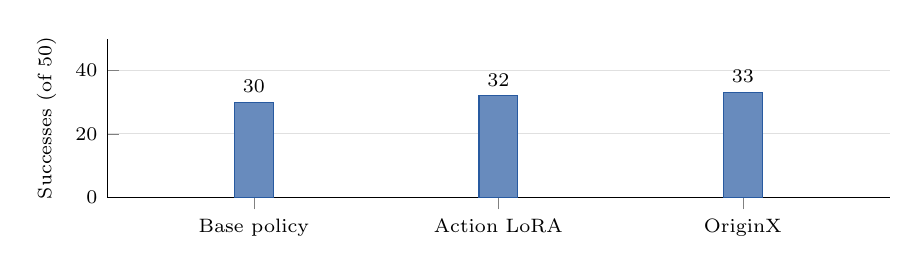
\begin{tikzpicture}
\begin{axis}[
  width=0.95\columnwidth, height=3.6cm,
  ybar, bar width=14pt, ymin=0, ymax=50,
  ylabel={Successes (of 50)}, ylabel style={font=\scriptsize},
  symbolic x coords={Base policy,Action LoRA,OriginX},
  xtick=data, tick label style={font=\scriptsize},
  nodes near coords, nodes near coords style={font=\scriptsize},
  enlarge x limits=0.3, axis lines*=left, ymajorgrids, grid style={black!12}]
\addplot[fill=edgeblue!70, draw=edgeblue] coordinates {(Base policy,30) (Action LoRA,32) (OriginX,33)};
\end{axis}
\end{tikzpicture}
\caption{Separate 50-case RoboCasa365 comparison of the adaptation study. On 44 matched LoRA/OriginX pairs: 5 wins, 4 losses, 35 ties (6 unresolved).}
\label{fig:robocasa}
\end{figure}

\subsection{OriginX-TF Engineering Checks}
The same harness, with identity-checked source code, perception front end, prompts and configuration, runs closed-loop RoboCasa episodes with both frozen policies and makes zero parameter updates. The test suite passes 145 CPU tests, with 2 skipped because of Windows symbolic-link permissions. For both backends, replaying the same static observations with and without moving the policy weights between CPU and GPU gave identical native actions, which supports the single-GPU sequential loading. These checks establish engineering feasibility and cross-backend reuse; they do not measure task success.

\subsection{OriginX-TF Pilot}
Twelve of the 14 planned episodes finished: 6 successes and 6 task failures; the other 2 are unknown (Fig.~\ref{fig:pilot}). These counts mix baselines and ablations and are not a success rate of the method. Xiaomi solved 1 of 2 tasks with or without the harness, and so did Awomo. Because the Xiaomi coffee-task episodes do not share a matched initial state with the full-harness episode, only three main pairs are valid, and all three show no difference. The no-stage and no-binding ablations each solved 1 of 2 tasks; both single-confirm episodes are unknown. In the cabinet task, where initial states match, the no-binding ablation succeeded at step 256 while the full harness failed at the 750-step limit. None of the four full-harness episodes committed a stage transition, and neither did the successful no-binding episode.

\begin{figure}[t]
\centering
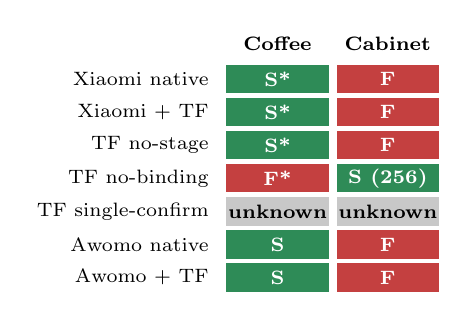
\begin{tikzpicture}[font=\scriptsize,
  cell/.style={minimum width=13mm, minimum height=3.6mm, inner sep=0pt, font=\scriptsize\bfseries}]
  \node[font=\scriptsize\bfseries] at (2.2,0.45) {Coffee};
  \node[font=\scriptsize\bfseries] at (3.6,0.45) {Cabinet};
  \foreach \name/\c/\cl/\k/\kl/\tc [count=\i] in {
    Xiaomi native/okgreen/S*/failred/F/white,
    Xiaomi + TF/okgreen/S*/failred/F/white,
    TF no-stage/okgreen/S*/failred/F/white,
    TF no-binding/failred/F*/okgreen/S (256)/white,
    TF single-confirm/unkgray/unknown/unkgray/unknown/black,
    Awomo native/okgreen/S/failred/F/white,
    Awomo + TF/okgreen/S/failred/F/white} {
    \node[anchor=east] at (1.45,-0.42*\i+0.42) {\name};
    \node[cell, fill=\c, text=\tc] at (2.2,-0.42*\i+0.42) {\cl};
    \node[cell, fill=\k, text=\tc] at (3.6,-0.42*\i+0.42) {\kl};
  }
\end{tikzpicture}
\caption{OriginX-TF (TF) pilot outcomes, one seed per task. S = success, F = failure; S (256) = success at step 256. * Coffee pairs with Xiaomi + TF are excluded from paired inference because its initial state does not match the other Xiaomi coffee episodes. The full harness failed the cabinet task at the 750-step limit.}
\label{fig:pilot}
\end{figure}

\section{Discussion (Partial)}
The midterm results separate what works from what is not yet shown. The data pipeline, the adapted policy and its large evaluation, and a harness that runs unchanged on two frozen policies on a single laptop GPU are complete. A task-success gain is not established: the adaptation study shows a small, uncertain difference, and the harness pilot shows no difference on its three valid main pairs.

The pilot logs point to a concrete bottleneck. Perception updates every 16 control steps, while a track expires after 30 steps without a match, so a single missed detection expires it; once the initial target ID expires, the harness has no path to rebind it and keeps falling back to the original instruction. Some verifier answers also mix the current stage with the final goal (for example, judging a grasp stage by the final placement). This is consistent with the absence of stage commits and with the matched cabinet case, where removing the identity gate (no-binding) succeeded even without a stage commit. One case, however, cannot establish a general effect in either direction.

The next version will (1) recover object identity after occlusion by distinguishing temporary invisibility, re-identification and target replacement; (2) ask the verifier only about the current postcondition and separate ``not done'' from ``uncertain''; and (3) record full initial-state components so that unmatched pairs can be diagnosed. We will first finish the 2 unknown pilot episodes with the unchanged version, then develop on the current cases, freeze the configuration, and evaluate on fresh held-out cases, reporting success rate, wrong-target commits, recoveries and inference cost. On the real robot, we will extend the folding and toolbox recordings and measure closed-loop success of the trained policies on the SO101 arm.

\section*{Acknowledgements}
We thank the ELEC 594 instructors for feedback on weekly reports, and H. Yang, J. Wu, S. Tang and G. Dai, co-authors of the OriginX study~\cite{ma2026originx}. AI assistants (OpenAI Codex and Anthropic Claude) were used for coding support, experiment orchestration, log analysis and drafting of this report; the author reviewed the content and is responsible for it. Code and evidence for the adaptation study are available at \url{https://github.com/Quinn-Ma/OriginX}.

\section*{CRediT Author Statement}
\textbf{Qinzhen Ma}: Conceptualization, Methodology, Software, Investigation, Data curation, Formal analysis, Visualization, Writing -- original draft, Writing -- review \& editing.

\bibliographystyle{IEEEtran}
\bibliography{refs}

\end{document}
